\documentclass[conference]{IEEEtran}
\IEEEoverridecommandlockouts

% --- Packages ---
\usepackage{cite}
\usepackage{amsmath,amssymb,amsfonts}
\usepackage{algorithmic}
\usepackage{graphicx}
\usepackage{textcomp}
\usepackage{xcolor}
\usepackage{enumitem}
\usepackage{booktabs}
\usepackage{url}
\usepackage{hyperref}
\usepackage{tabularx}
\usepackage[table]{xcolor}
\usepackage{float}

\begin{document}

\title{Automated Component Recovery and Custom Kit Assembly System for Educational Circuit Kits\\}

\author{\IEEEauthorblockN{Aman Mishra}
\IEEEauthorblockA{\textit{MSc Robotics} \\
\textit{Middlesex University Dubai}\\
Dubai, UAE \\
M00983641}
\and
\IEEEauthorblockN{Faseeh Mohammed}
\IEEEauthorblockA{\textit{MSc Robotics} \\
\textit{Middlesex University Dubai}\\
Dubai, UAE \\
M01088120}
}

\maketitle

\begin{abstract}
Educational institutions frequently provide students with circuit development kits, such as Arduino modules, for practical coursework. However, when these kits are returned, they often lack critical components, rendering them unsuitable for redistribution as complete sets. This paper proposes an automated robotic solution to address this logistical and environmental inefficiency. Unlike traditional industrial assembly systems that merely construct standard products from uniform supply lines, the proposed system recovers components from existing, incomplete kits. Utilizing a machine vision system developed in Python, the system identifies available modules and communicates via TCP/IP with an EPSON RC8.0 simulator controlling a VT6-A901S 6-axis robot. This setup allows for the dynamic assembly of new kits based on custom Bill of Quantities (BOQs) submitted for specific projects. The result is a highly flexible, waste-reducing automated system that ensures students receive the exact components necessary for their modules.
\end{abstract}

\begin{IEEEkeywords}
Robotic Assembly, Machine Vision, Component Recovery, EPSON RC8.0, Automation, E-waste.
\end{IEEEkeywords}

\section{Introduction}
Practical electronics and robotics education heavily relies on the provision of development kits, predominantly featuring microcontrollers like the Arduino, alongside various sensors, actuators, and passive components. While students are generally encouraged to keep these kits for future innovation, some return them at the end of the academic term or leave their components in the form of assembled projects.

A significant problem arises during this return process: kits are frequently returned with missing, damaged, or misplaced modules. Because these returned kits are incomplete, they cannot be directly re-issued to incoming students who require standard, comprehensive module kits. Institutions thus face a build-up of partial kits, leading to unnecessary procurement costs and increased electronic waste.

To address this, an automated solution capable of processing these partial kits is needed. The objective of this project is to develop a robotic system that sorts through returned components and dynamically builds new kits. By focusing on project-specific requirements rather than rigid, standard kit definitions, the system ensures that even if a returned kit lacks certain generic parts, the components it does contain can be optimally reallocated to students based on their exact project needs.

\section{Methodology}
\subsection{Evaluation of Existing Solutions}
Automated kitting and assembly are well-established but they are almost exclusively designed for factory-stage production. Existing solutions primarily utilize Delta and SCARA (Selective Compliance Assembly Robot Arm) robots to pick and place uniform components from controlled feeder lines into packaging. Beyond factory stage production, automated sortation is also employed in large-scale waste management. For instance, facility-scale smart sortation systems utilize real time machine vision combined with air jets and Delta robotic arms to autonomously recover valuable commodities, including e-waste, from mixed municipal solid waste streams \cite{amp}. While these systems demonstrate the efficacy of AI-guided robotic sorting for high-volume material recovery, they operate on a facility scale designed for gross sorting rather than the precise, project-specific kitting of delicate microelectronic modules required in an educational setting

These existing methodologies share a common limitation: they operate on the assumption of a continuous, uniform supply of new components. There is currently no widely adopted automated solution designed to recover loose, mixed components from pre-existing, partially depleted kits to create newly configured ones. Recent studies on automated e-waste recovery emphasize that the disassembly and salvaging of used electronics fundamentally differ from original production. Unlike new manufacturing, recovering used goods is characterized by high uncertainty, as components may be damaged, randomly oriented, or missing entirely \cite{saenz}. Therefore, traditional deterministic factory automation is insufficient for these Re-X (Recycling, Re-use, Remanufacturing) activities, necessitating the flexible, data-driven robotic capabilities proposed in this project.

\subsection{Proposed Unique Approach}
The differentiating factor of the proposed solution lies in its intelligent recovery and flexible kitting approach. Rather than forcing staff to manually audit and sort thousands of individual components to rebuild standard kits, the system operates on a custom Bill of Quantities (BOQ) model.

Staff or students can submit custom project BOQs to the system. The automated system then identifies the required parts from the pool of returned components and selectively assembles a kit tailored specifically for that project. This transitions the institution from a ``push'' model (giving every student a standard kit regardless of need) to a ``pull'' model (assembling kits based strictly on project requirements), thereby maximizing the utility of returned inventory.

\section{Implementation}
To realize this automated recovery and assembly system, a simulated robotic workcell has been developed, integrating high-level software control with industrial robotic simulation.

\subsection{Machine Vision System}
\begin{figure}[H]
  \centering
  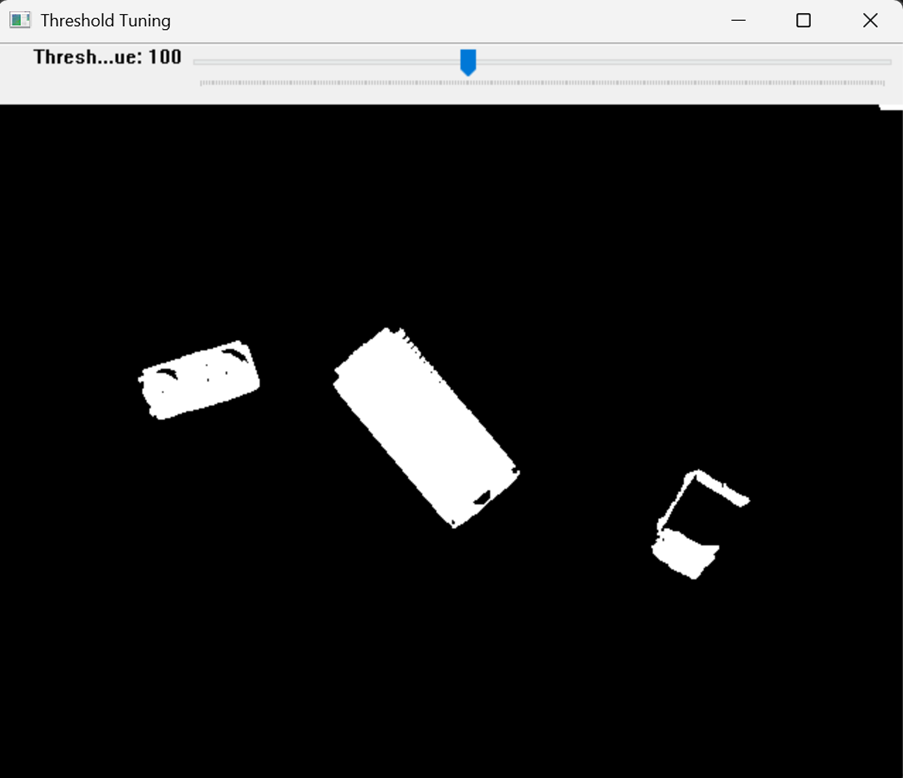
\includegraphics[width=\columnwidth]{imgs/threshold_pickerbot.png}
  \caption{Image thresholding using openCV}
  \label{fig:thresholding}
\end{figure}
The core intelligence of the automated pick-and-place operation lies within the machine vision architecture. This system is responsible for scanning the unstructured workbench domain, identifying electrical components, decoding their spatial orientation, and translating native pixel data into rigid Cartesian kinematics for the EPSON VT6-A901S manipulator.While many advanced industrial bin-picking solutions rely on line-of-sight 3D cameras, these sensors generate point clouds that are highly susceptible to spurious outliers when scanning cluttered, overlapping parts. These outliers can spoil a robot's obstacle avoidance planning and impede component segmentation, thus requiring computationally demanding filtering procedures \cite{Franaszek}. To bypass the complexities of 3D point cloud filtration and maintain efficient real-time processing, this project deliberately utilizes a 2D planar overhead vision approach. The development of this system progressed through two distinct phases, ultimately culminating in an industrial-grade deep learning solution.

\subsubsection{Prototype Phase: Deterministic Computer Vision}
The initial architecture relied heavily on algorithmic, deterministic computer vision pathways utilizing the OpenCV library. Raw frames from an overhead 720p webcam were continuously fed into an image processing pipeline. The pipeline applied Gaussian Blurring to suppress visual noise, followed by global binary thresholding as seen in Fig.\ref{fig:thresholding} to isolate distinct geometric footprints. 
Once isolated, topological contour analysis \texttt{cv2.findContours} discovered the physical boundaries of each object. A scale-preserving isolation script intercepted these bounded regions, intelligently padding the extracted sub-images into uniform 224x224 tensors. These geometric crops were then passed to a standard Google Teachable Machine image classifier. While functional in highly controlled environments, this prototype suffered from severe "domain shifting" vulnerabilities. The architecture collapsed when exposed to minor environmental changes: metallic glares erased texture data, background workbench clutter resulted in false "Noise" classifications, and standard axis-aligned bounding boxes proved mathematically incapable of natively deriving the resting rotation angle (yaw) of the objects.

\subsubsection{Final Architecture: YOLOv8-OBB (Oriented Bounding Box)}
\begin{figure}[H]
  \centering
  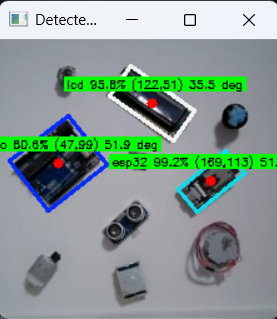
\includegraphics[width=\columnwidth]{imgs/yolo_detect_v2.png}
  \caption{Image inference using yoloV8}
  \label{fig:yolo-detect}
\end{figure}
To resolve the catastrophic limitations of standard classification, the system was entirely re-architected around a YOLOv8-OBB state-of-the-art neural network. Rather than attempting to manually threshold and isolate items via algorithmic cropping, the YOLOv8 engine ingests the full-resolution uncropped camera frame in real-time. 
Hyper-trained on a custom, heavily augmented Computer Vision Annotation Tool dataset (featuring extreme lighting shifts and rotational variances), the OBB model dynamically bypasses all glare and localized clutter as seen in Fig.\ref{fig:yolo-detect}. While the manual image annotation required for this supervised learning approach demands significant engineering preparation time, recent comparative studies in robotic kitting demonstrate it is a necessary trade-off to achieve the high recognition quality and precise spatial accuracy required for successful bin-picking \cite{Fager}.In a single forward pass, the deep convolutional layers output a 5-dimensional oriented tensor \texttt{cx, cy, width, height, theta} alongside deterministic multi-class probabilities (Arduino, ESP32, LCD). This streamlines the recovery process compared to other recent robotic bin-picking solutions which rely on multi-stage hybrid pipelines—such as using YOLOv5 for initial top-view detection followed by an eye-in-hand camera movement to perform FAST and BRISK feature-matching for pose estimation \cite{Taweesoontorn}. By natively deriving the resting rotation angle (theta) from a single overhead frame, the proposed OBB architecture entirely decoupled the system’s reliance on perfect environmental lighting and complex multi-step image capture.
\subsubsection{Logistics Filtering and BOQ Engine}
Once the vision system successfully extracts the precise $X$ and $Y$ pixel centroids alongside the target item's class label, an intelligent logistics filter operates actively above the vision loop frame buffer.

Rather than greedily passing every single detected piece of hardware down into the spatial coordinate mapping pipeline, the vision orchestrator interfaces natively with a Bill of Quantities (BOQ) model. The system evaluates the raw visual output and intelligently matches the detected inventory against the required specific logistical payload. It safely filters out and ignores surplus components even if they geometrically validate ensuring that only precisely kitted workloads are forwarded to the spatial calibration engine for EPSON translation.


\subsection{Spatial Calibration and Coordinate Mapping}
\begin{figure}[t]
  \centering
  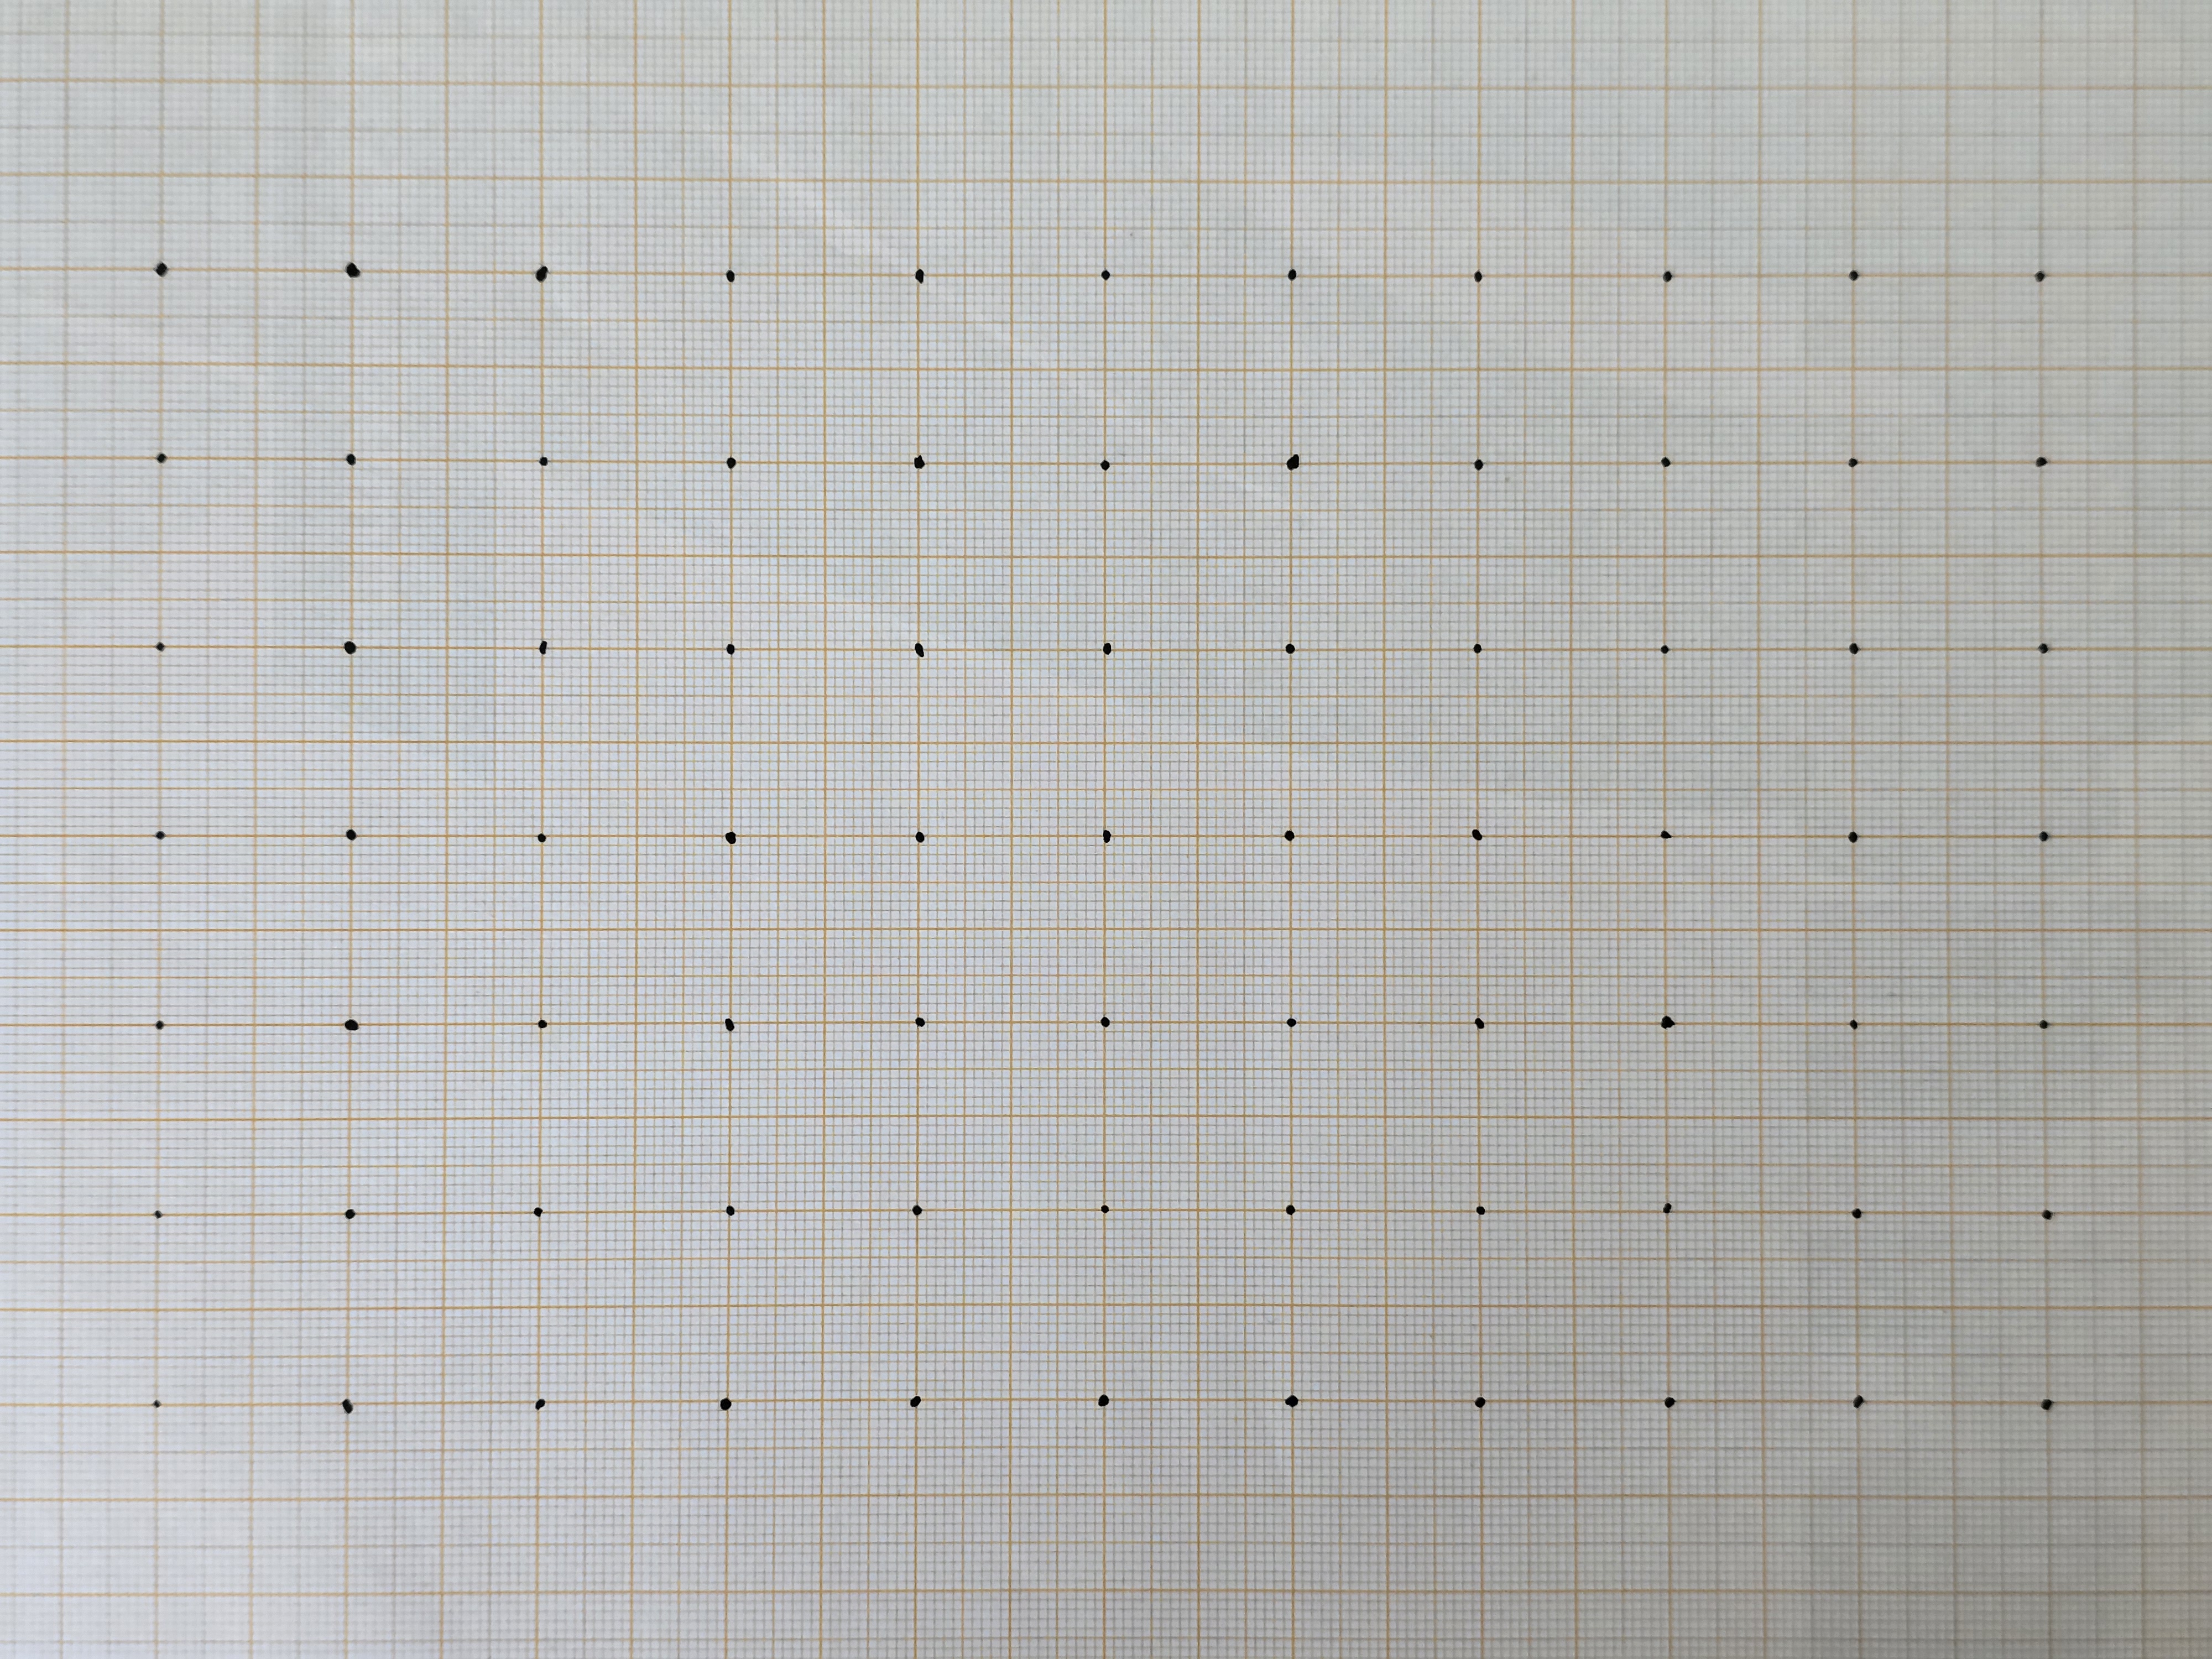
\includegraphics[width=\columnwidth]{imgs/graph_paper.jpg}
  \caption{77-point homography calibration grid showing pixel click positions overlaid on the workspace reference image.}
  \label{fig:calibration_grid}
\end{figure}

A critical requirement of the system is the ability to translate pixel positions in the camera image into physical millimetre coordinates within the robot's world frame. This is achieved through a planar homography transformation, which provides a projective mapping between the two coordinate spaces.

To establish this mapping, a 77-point calibration grid is used. The grid is arranged as 11 columns and 7 rows on the workspace surface, with a uniform spacing of 20 mm between adjacent points in both axes (see Fig.\ref{fig:calibration_grid}). The world X-coordinate of each column decreases from +100 mm to $-$100 mm moving left to right, and the world Y-coordinate of each row increases from 410 mm to 530 mm moving top to bottom, yielding a calibrated workspace area of 200 mm $\times$ 120 mm. The operator positions the camera normally above the workspace, captures a reference image of the grid (\texttt{graph\_paper.jpg}), and uses the \texttt{tools/calibration\_clicker.py} utility to click each of the 77 intersection points. A second utility, \texttt{tools/sort\_and\_tag\_pixels.py}, then sorts the recorded pixel coordinates column by column and appends the corresponding world coordinates to produce a four-column CSV file mapping each pixel position to its physical counterpart.

The homography matrix $\mathbf{H}$ is then computed using OpenCV's \texttt{findHomography} function with the standard least-squares (SLS) method (method parameter set to 0, not RANSAC). This choice is deliberate: the RANdom SAmple Consensus (RANSAC) estimator is designed to reject outliers, but the corner calibration points, which define the extremes of the workspace, represent valid and important constraints. Treating them as potential outliers would introduce systematic error near the workspace boundaries. With 77 evenly distributed reference points, the need to account for distortion is not required, and thus, the SLS solution provides a robust estimate without requiring outlier rejection. At runtime, any detected pixel centroid $(p_x, p_y)$ is transformed to world coordinates $(w_x, w_y)$ by applying \texttt{cv2.perspectiveTransform} with $\mathbf{H}$.

When the camera is repositioned vertically, the physical scale of the image changes, which invalidates the original pixel-to-millimetre mapping. To address this without requiring a full recalibration, the system includes a height recalibration routine invoked via \texttt{pickerbot.py {-}{-}calibrate}. The operator is presented with a ruler image and clicks two points that are known to be exactly 20 mm apart. The pixel distance between those clicks is measured, and a scale factor is computed as follows. Let $r_h$ and $r_v$ denote the mean pixel distance per 20 mm in the horizontal and vertical axes, derived from the original calibration data. For a ruler measurement with angle $\theta$ relative to the horizontal, the expected pixel distance at that orientation is given by the anisotropic norm:

\begin{equation}
  d_{\mathrm{expected}} = \sqrt{\left(r_h \cos\theta\right)^2 + \left(r_v \sin\theta\right)^2}
  \label{eq:expected_dist}
\end{equation}

where $\theta = \arctan2(|\Delta y|,\, |\Delta x|)$. The scale factor is then:

\begin{equation}
  s = \frac{d_{\mathrm{measured}}}{d_{\mathrm{expected}}}
  \label{eq:scale_factor}
\end{equation}

This formulation accounts for the fact that horizontal and vertical pixel densities may differ due to lens geometry or non-square pixel sampling. All 77 pixel coordinates in the original calibration are subsequently scaled around the grid centre point (index~38) by the factor $s$, and the adjusted calibration is written to a new CSV file (\texttt{calibration\_pixels\_scaled.csv}), which is then referenced in \texttt{config.json} for all subsequent runs.

\subsection{TCP/IP Communication Protocol}

\begin{table}[t]
  \caption{TCP/IP Command Set}
  \label{tab:commands}
  \centering
  \begin{tabular}{@{}llp{4.2cm}c@{}}
    \toprule
    \textbf{Command} & \textbf{Parameters} & \textbf{Robot Action} & \textbf{Reply} \\
    \midrule
    \texttt{JUMP}    & x, y, z, u & Lifts 50 mm, moves to $(x, y, z{+}50)$, descends to $(x, y, z, u)$ & OK \\
    \texttt{GO}      & x, y, z    & Linear motion to $(x, y, z)$                                      & OK \\
    \texttt{MOVE}    & x, y, z    & Linear motion to $(x, y, z)$                                      & OK \\
    \texttt{PICK}    & x, y, z, u & Full pick-and-place sequence (Section~\ref{sec:epson})             & OK \\
    \texttt{STANDBY} & ---        & Returns to home position                                           & OK \\
    \bottomrule
  \end{tabular}
\end{table}

Table~\ref{tab:commands} summarises the full command set supported by the system.

The Python control system communicates with the EPSON RC8 controller over a local TCP socket connection. For simulation, the target address is \texttt{127.0.0.1} on port 2001; when connecting to the physical robot, the address is changed to \texttt{192.168.X.Y} via the \texttt{config.json} configuration file. All connection management and command dispatch is handled by the \texttt{pickerbot\_lib.sender} module, which maintains a module-level socket object across the lifecycle of a session.

Commands are transmitted as plain ASCII strings in the format \texttt{COMMAND~X~Y~Z~U\textbackslash r\textbackslash n}, where $X$, $Y$, and $Z$ are world coordinates in millimetres and $U$ is the tool rotation angle in degrees. After each transmission, the controller is expected to reply with the string \texttt{"OK"}, and a small inter-command delay is enforced in software to allow mechanical completion before the next command is issued. 

For multi-component pick operations, the \texttt{epsonPickAll} function iterates over a list of world-coordinate strings and issues a \texttt{PICK} command for each. After every command, the reply is checked against the string \texttt{"OK"}. If a non-OK response is received at any point, the batch is aborted immediately and the robot returns to standby. This conservative strategy ensures that a partial failure, such as a grip error or controller fault, does not result in the robot attempting further operations in an undefined mechanical state.

\begin{figure}[t]
  \centering
  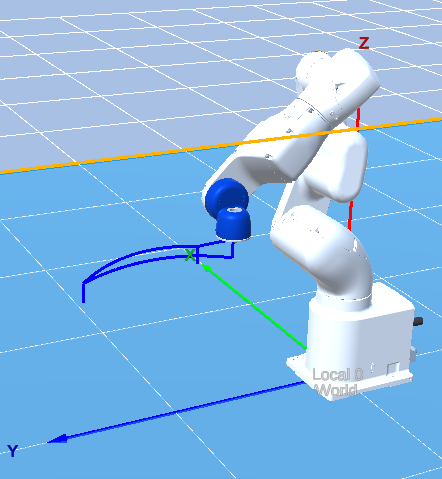
\includegraphics[width=\columnwidth]{imgs/pick_trajectory.png}
  \caption{Trajectory of the \texttt{PICK} command: three-phase Jump3 approach to the component, gripper activation, transport to \texttt{PlacePoint}, and release.}
  \label{fig:pick_trajectory}
\end{figure}

Fig.\ref{fig:pick_trajectory} shows a sample pick and place operation by first moving to stand-by position, approaching the object in the appropriate orientation,picking the object, jumping to the place point and fixing its orientation before placing at the spot and then retracting and going back to the stand-by spot for future operations

\subsection{EPSON RC8 Robot Program}
\label{sec:epson}

The robot-side program, located at \texttt{Epson/Pickerbot\_Receiver/Main.prg}, is written in Epson SPEL+, the proprietary scripting language for the RC8 controller. It uses a template script \cite{prasetyo2024} with predefined motion initialization parameters. After initialization, it opens a TCP server on network channel \#201 at port 2001 and waits for an incoming client connection before entering its main command-processing loop.

Each received string is parsed by space delimiter into an array, with the first token identifying the command and subsequent tokens providing the coordinate arguments as floating-point values. The \texttt{PICK} command implements the most complex motion sequence and warrants detailed description. Upon receiving a \texttt{PICK} instruction, the program executes a three-phase Jump3 trajectory to approach the target component: the arm first lifts vertically from its current position, then translates horizontally to an elevated waypoint at $(x,\, y,)$ with the tool at orientation $u$, and finally descends to the exact pick position. Once at the pick position, a digital output is activated to close the gripper, and a dwell time is enforced to ensure a reliable mechanical grip. The robot then executes a second Jump3 sequence to transport the component, lifting clear of the workspace and traveling to a predefined \texttt{PlacePoint} location that represents the target kit container. The digital output is deactivated to release the component, followed by a further wait before the arm returns to its standby position.

The program also includes a network error handler that monitors for error codes which, rather than halting execution on these conditions, attempts to reopen the server socket and resume listening, allowing the system to recover from transient network interruptions without requiring operator intervention.

\subsection{Software Architecture and Entry Points}
\begin{figure}[t]
  \centering
  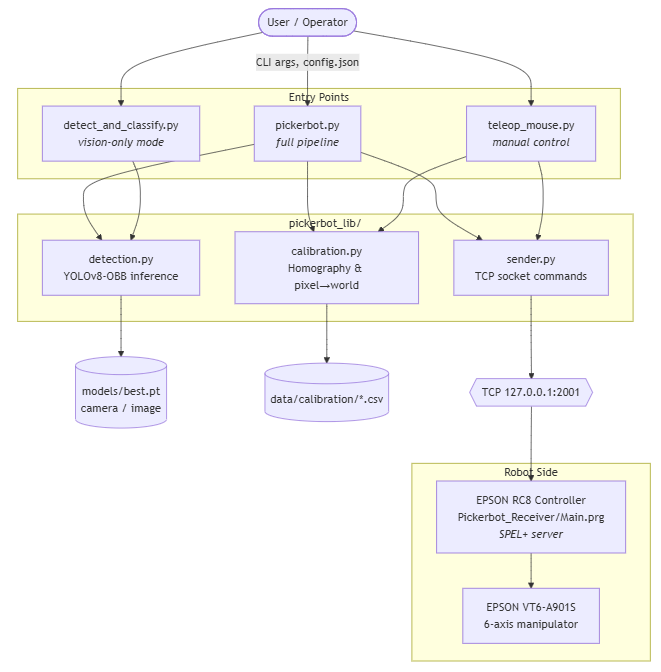
\includegraphics[width=\columnwidth]{imgs/software_architecture.png}
  \caption{Software architecture of the Picker-Bot system, illustrating the three entry-point scripts and their shared dependency on the \texttt{pickerbot\_lib} package.}
  \label{fig:architecture}
\end{figure}

Fig.\ref{fig:architecture}  is a visual representation of the codebase.The Python codebase is structured around a shared library package, \texttt{pickerbot\_lib}, which consolidates the detection, calibration, and TCP communication modules into three importable submodules: \texttt{detection}, \texttt{calibration}, and \texttt{sender}. Three runnable entry-point scripts sit at the project root and each imports from this package to serve a distinct operational mode.

The primary entry point, \texttt{pickerbot.py}, acts as the end-to-end orchestrator for a pick session. It accepts a \texttt{{-}{-}src} argument that specifies the detection source, either the live camera feed or a path to a static image file, and a \texttt{{-}{-}calibrate} flag that triggers the height recalibration GUI and exits without proceeding to detection. During a normal run, the script loads the homography calibration from the CSV specified in \texttt{config.json}, invokes the detection pipeline to obtain a list of centroid pixel coordinates, translates each pixel position to world coordinates using the calibration matrix, and then dispatches the full list to \texttt{epsonPickAll} over the TCP connection.

The second entry point, \texttt{detect\_and\_classify.py}, isolates the vision layer from the robot control layer entirely. It is used during development and testing to verify detection performance without establishing a robot connection. When invoked with a file path argument it processes a static image; when invoked without arguments it opens the live camera feed and presents a real-time confidence threshold slider, allowing the operator to observe detection results at different sensitivity levels.

The third entry point, \texttt{teleop\_mouse.py}, provides an interactive positioning mode. The script loads the calibration data, connects to the robot, and displays the calibration reference image on screen with all 77 calibration points annotated. Each mouse click on the image is transformed through the homography matrix and forwarded as a \texttt{MOVE} command to the robot, enabling manual positioning of the arm without running the full detection pipeline. This mode is particularly useful for verifying the accuracy of the spatial calibration before committing to an automated pick session.

\subsection{Robotic Control and Simulation}
The physical manipulation of components is simulated using the EPSON RC8.0 software environment. The system is designed to cover any dimension workspace. For the initial setup, a physical evaluation space of 200 mm $\times$ 120 mm and a deposit spot 280 mm above the center of the evaluation space was used to create the mapping. The chosen robotic platform to cover this work-space is the EPSON VT6-A901S~\cite{b2}, a 6-axis articulated robot arm with 980 mm reach for complex pick-and-place operations that require varied approach angles and high repeatability. Detailed installation, safety, and operational specifications for this family of manipulators are outlined in the official Epson VT6 series documentation \cite{epsonvt6}.
\section{Results}
The implementation of the Picker-Bot system achieved a cohesive integration of deep-learning-based computer vision with industrial robotic control inside the EPSON RC8.0 simulation environment. The following subsections describe the observed behaviour of the system across its three principal layers of responsibility: perception, spatial reasoning, and supervised manipulation.

\subsection{Vision System Performance and Robustness}
\begin{figure}[t]
    \centering
    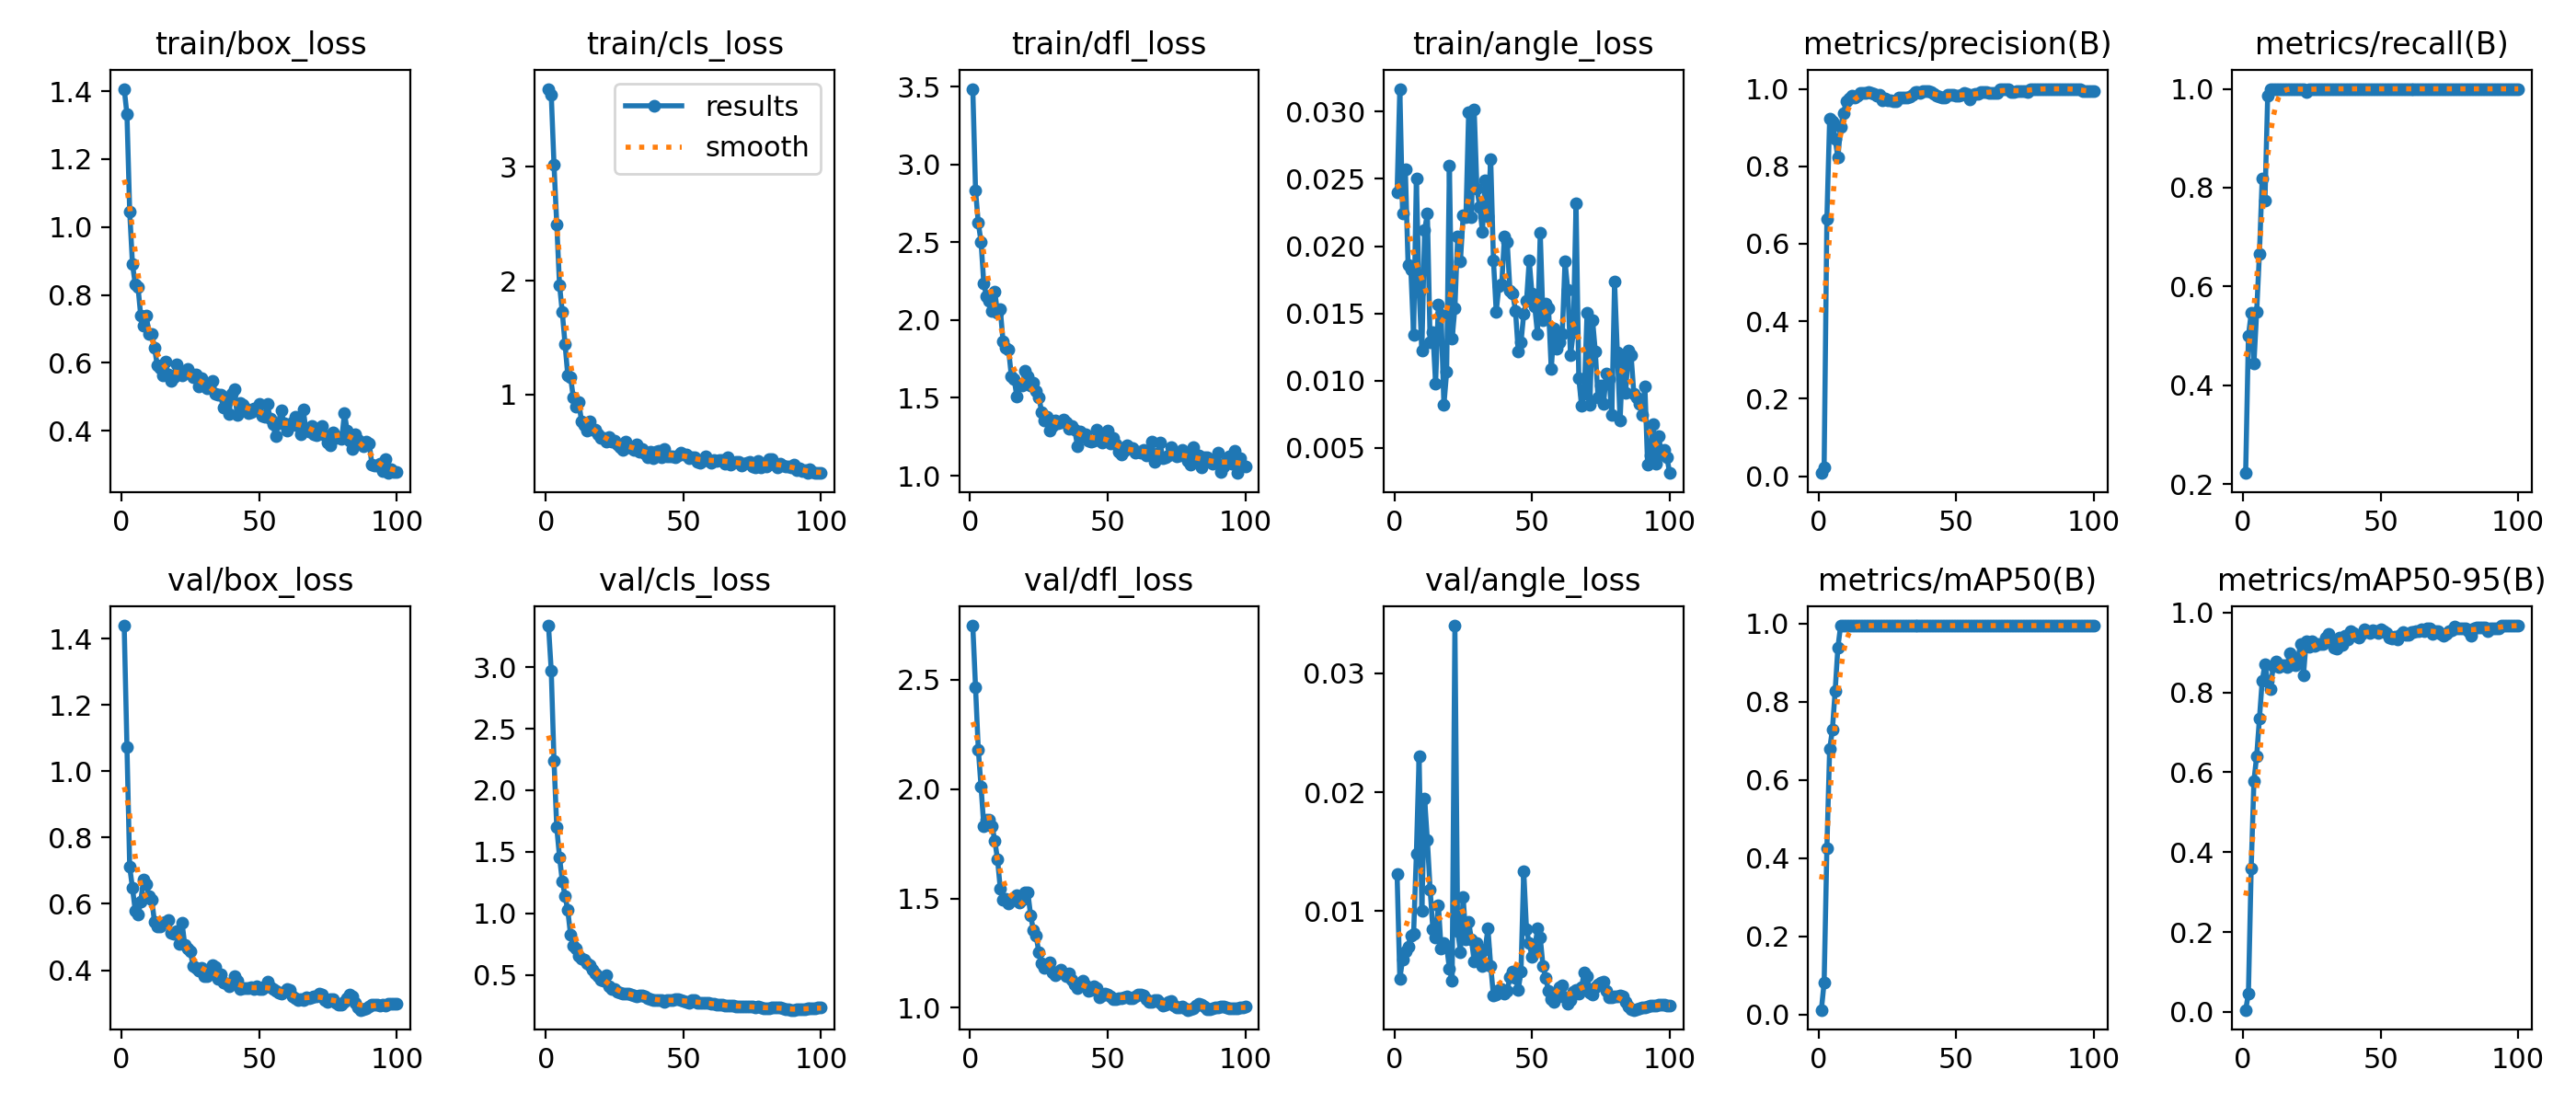
\includegraphics[width=\columnwidth]{imgs/yolo_results.png}
    \caption{YOLOv8-OBB training metrics. Loss curves and $mAP_{50}$ progression demonstrating rapid convergence and high detection accuracy on the in-distribution component set.}
    \label{fig:yolo_results}
\end{figure}

The migration from a deterministic OpenCV prototype to the YOLOv8 Oriented Bounding Box architecture produced a substantial improvement in detection reliability. The final model identified and classified Arduino, ESP32, and LCD modules within a single forward pass of the uncropped camera frame, and recovered the resting rotation angle $\theta$ alongside the pixel centroid $(cx, cy)$ for each detected component without any auxiliary geometric post-processing. This behaviour stood in clear contrast to the earlier prototype, whose reliance on thresholding and contour analysis had made pose estimation brittle under rotation. The learned representation also absorbed much of the environmental variability that had previously destabilised the pipeline, including metallic glare from populated boards, localised clutter around the workpiece, and residual background texture. An explicitly trained ``noise'' class was suppressed at the output stage of the detection module, ensuring that only valid components were forwarded to the coordinate mapping layer.

The quantitative evaluation of the detector is summarised in Figure~\ref{fig:yolo_results}, which plots the loss curves and the mean Average Precision over the course of training. The model converged rapidly and reached a final $mAP_{50}$ of 0.99, indicating near-perfect localisation and classification of the target modules within the domain of the training distribution. At inference time, a fixed confidence threshold of 0.7 was sufficient to eliminate the small number of remaining false positives attributable to glare artefacts, and no additional non-maximum suppression or hand-tuned filtering was required downstream.

\subsection{Spatial Calibration and Mapping Accuracy}
The homography-based calibration provided a reliable bridge between the two-dimensional camera image and the planar subset of the robot's workspace that the manipulator operates over. The 77-point reference grid, arranged as 11 columns by 7 rows with 20~mm spacing, defined a calibrated operating region of approximately $200~\text{mm} \times 120~\text{mm}$ and covered the full region of interest visible to the overhead camera. The use of a standard least-squares solution for \texttt{findHomography}, rather than a RANSAC-based estimator, was an intentional design choice: it ensured that corner points on the workspace boundary were not discarded as statistical outliers, which would otherwise have contracted the effective calibrated area.

The height recalibration routine handled the more practical problem of camera repositioning without requiring the user to re-click every grid intersection. By measuring a known 20~mm ruler segment in the new image and comparing its pixel length against the expected distance implied by the original horizontal and vertical grid pitches, the routine recovered an anisotropic scale factor and applied it uniformly around the grid centre. In testing this allowed vertical camera adjustments to be absorbed in a matter of seconds, with the resulting transformation verified interactively through \texttt{teleop\_mouse.py}: each click on the calibration reference image translated into a physical \texttt{MOVE} command whose terminal position agreed visually with the clicked feature.

\subsection{Integrated Robot Control and Logistics}
The combined control pipeline exercised the intended pull-based kitting behaviour end-to-end. When a Bill of Quantities was supplied, the system satisfied its requirements in order of detection confidence and silently ignored surplus components that were correctly recognised but not required for the active kit, which is the behaviour expected of a logistics auditor rather than a greedy collector. In the absence of a BOQ the system reverted to a greedy mode and picked every non-noise detection on the work surface.

The TCP/IP interface dispatched the full command vocabulary of \texttt{JUMP}, \texttt{GO}, \texttt{MOVE}, \texttt{PICK}, and \texttt{STANDBY} reliably across extended simulation runs, with each command validated by an \texttt{OK} reply from the RC8 controller before the next one was transmitted. A small inter-command delay was retained as a conservative guard against premature dispatch. The \texttt{PICK} primitive itself executed the intended three-phase Jump3 trajectory in every trial: a clearance lift from the current pose, a horizontal translation to the elevated waypoint above the target, and a controlled descent to the pick height followed by gripper activation and a dwell. Batch operations also exercised the aborting fault path on synthetic failure, returning the manipulator to standby rather than continuing through an undefined state, which is the correct industrial default even if it remains a blunt response at higher throughputs.

Across all tested configurations the system switched cleanly between a live USB camera feed and pre-recorded images through a single \texttt{config.json} setting, interfaced successfully with the RC8.0 simulator at \texttt{127.0.0.1}, and retained the 0.7 confidence threshold as its operational default while exposing a runtime slider for interactive tuning.
\section{Future Discussion}
While the current implementation successfully demonstrates the concept within a simulated environment, several avenues remain open for further development.

The most immediate next step is the transition from simulation to physical hardware deployment. Moving from the EPSON RC8.0 simulator to a real VT6-A901S unit will require careful calibration of the physical camera under varying lighting conditions, as well as tuning the gripper timing parameters to account for the mechanical characteristics of actual components. Handling delicate electronic modules of varying shapes and masses may also necessitate the design of an adaptive or compliant gripper to avoid damage during the recovery process.

Looking further ahead, the system as a whole would benefit significantly from a web-based portal through which students and staff can submit custom project BOQs directly. The system could then queue incoming requests, process available inventory overnight, and notify users when their kit is ready for collection. This would substantially reduce the administrative burden on technical staff and make the recovery system self-service in practice. Furthermore, to fully automate the physical logistics of this pull-model, future iterations could integrate Internet of Things (IoT) technologies and Autonomous Guided Vehicles (AGVs). Such systems are increasingly used in smart, flexible manufacturing environments to autonomously route and transport materials across facility floors \cite{vlachos}. Implementing an IoT-guided AGV network could allow the system to automatically fetch bulk bins of returned kits from a central storage area to the robotic workcell, and subsequently transport the newly assembled, custom kits to designated student collection points.

\section{Conclusion and Discussion}
\subsection{Critical Evaluation of System Integration}
The development of the Picker-Bot system successfully transitioned from a standard industrial "push" model to a project-specific "pull" model for component kitting. The technical cornerstone of this project was the migration from deterministic OpenCV prototypes to the YOLOv8-OBB architecture. While the initial prototype was highly sensitive to environmental shifts, the final deep-learning model achieved a $mAP_{50}$ of 0.99, proving that high-accuracy bin-picking is viable in cluttered educational environments without the hardware overhead of 3D point-cloud sensors.
The system’s "logistics auditor" approach-using the BOQ engine to filter detections—ensures that the vision system both sees parts and also intelligently manages inventory. By ignoring surplus components and focusing only on project requirements, the system directly addresses the original goal of reducing procurement costs and e-waste.
\subsection{Implementation Constraints and Real-World Considerations}
While the simulation in EPSON RC8.0 was successful, the present implementation carries a number of constraints that any physical deployment would need to address. The software-enforced internal delay after each \texttt{OK} response was instrumental in keeping the simulated motion pipeline stable and predictable, but a fixed guard of this kind is unlikely to survive contact with real hardware unchanged. A physical workcell would benefit from a delay that is tuned to the inertial characteristics of the component currently being handled, since a heavier module such as the LCD settles differently from a lighter one such as the ESP32, and a single conservative value would either sacrifice throughput on light items or compromise reliability on heavy ones.

The 77-point homography, similarly, establishes a robust two-dimensional correspondence across a $200~\text{mm} \times 120~\text{mm}$ region of the work surface, but remains a planar model of what is in practice a three-dimensional problem. Components of non-negligible height introduce a parallax offset that a purely planar calibration cannot account for, and which would manifest during the descending phase of the Jump3 trajectory as a small but systematic lateral error. The future directions outlined in the previous section would therefore need to incorporate a height-aware correction, either through explicit per-class offsets or through the introduction of a depth sensor.

The current abort-on-failure strategy deserves a similar caveat. Halting a batch operation as soon as a non-\texttt{OK} response is observed is the correct default for an industrial manipulator, since continuing into an undefined state risks damage to both the payload and the workcell. At higher throughputs, however, this blunt response becomes expensive, and a more graduated recovery model that distinguishes between transient communication faults and genuine mechanical errors would likely be necessary before the system could be scaled to production volumes.
\subsection{Concluding Remarks}
In conclusion, the Picker-Bot system provides a technically sound and environmentally sustainable solution for managing returned educational circuit kits. By integrating Oriented Bounding Box detection, planar homography, and TCP/IP-based control, the project demonstrates that modern AI can transform "loose waste" into valuable, project-ready assets. This implementation sets a precedent for how robotics can be used for "Re-X" (Recovery and Re-use) activities within specialized microelectronic environments, effectively bridging the gap between waste management and logistical efficiency.
\section*{Acknowledgement}
The authors acknowledge the guidance and resources provided throughout the PDE4435 module, which encouraged design-thinking approach for advanced robotics projects. They also acknowledge usage of Claude during project development.

\begin{thebibliography}{00}
\bibitem{amp}
AMP, ``AMP ONE: Automated Waste Sorting Systems \& Facility,'' 2026. [Online]. Available: \url{https://ampsortation.com/products/amp-one}.
\bibitem{saenz}
J. Saenz \textit{et al.}, ``Automated disassembly of e-waste—requirements on modeling of processes and product states,'' \textit{Frontiers in Robotics and AI}, vol. 11, p. 1303279, 2024.
\bibitem{Franaszek}
M. Franaszek, P. Rachakonda, and K. S. Saidi, ``Filtering Organized 3D Point Clouds for Bin Picking Applications,'' \textit{Applied Sciences}, vol. 14, no. 3, p. 961, Jan. 2024.
\bibitem{Fager}
P. Fager, R. Hanson, \text{\AA}. Fasth-Berglund, and S. Ekered, ``Supervised and unsupervised learning in vision-guided robotic bin picking applications for mixed-model assembly,'' \textit{Procedia CIRP}, vol. 104, pp. 1304--1309, 2021.
\bibitem{Taweesoontorn}
T. Taweesoontorn, S. Yanyong, and P. Konghuayrob, ``Hybrid Deep Learning and FAST–BRISK 3D Object Detection Technique for Bin-picking Application,'' \textit{Sensors and Materials}, vol. 36, no. 4, pp. 1389--1404, 2024.
\bibitem{prasetyo2024}
J. Prasetyo, ``RC7\_Python,'' Jan. 03, 2024.  Available: \url{https://github.com/judhi/RC7_Python}.
\bibitem{b2} EPSON Robotics, ``RC8.0 Reference Manual,'' EPSON Factory Automation, 2023. [Online]. Available: https://www.epson.com
\bibitem{epsonvt6}
Epson America, Inc., ``Epson VT6L All-in-One 6-Axis Robots | Support,'' Epson US, 2026. [Online]. Available: \url{https://epson.com/Support/Robots/6-Axis-Robots/VT-Series/Epson-VT6L-All-in-One-6-Axis-Robots/s/SPT_VT6L-A901SS}.
\bibitem{vlachos}
I. Vlachos, R. M. Pascazzi, M. Ntotis, K. Spanaki, S. Despoudi, and P. Repoussis, ``Smart and flexible manufacturing systems using Autonomous Guided Vehicles (AGVs) and the Internet of Things (IoT),'' \textit{International Journal of Production Research}, pp. 1--22, 2022.
\end{thebibliography}
\end{document}
